\documentclass{article}
\usepackage[utf8]{inputenc}
\usepackage[spanish]{babel}
\usepackage{listings}
\usepackage{graphicx}
\graphicspath{ {images/} }
\usepackage{cite}

\begin{document}

\begin{titlepage}
    \begin{center}
        \vspace*{1cm}
            
        \Huge
        \textbf{Parcial II 2021-1 Informática 2}
            
        \vspace{0.5cm}
        \LARGE
        Informe de Implementación de la Solución del Desafío
            
        \vspace{1.5cm}
            
        \textbf{Juan Diego Cabrera Moncada}\\
            
        \vfill
            
        \vspace{0.8cm}
            
        \Large
        Despartamento de Ingeniería Electrónica y Telecomunicaciones\\
        Universidad de Antioquia\\
        Medellín\\
        Septiembre de 2021
            
    \end{center}
\end{titlepage}

\tableofcontents
\newpage
\section{Clases implementadas}
Las clases implementadas para el presente proyecto, corresponde a la clase QImage, con la cual un objeto de dicha clase es capaz de almacenar una imagen al obtener su dirección y tanto leer (Método pixelColor) como modificar el color de cada pixel que hace parte de la imagen y, asimismo, también puede obtener el valor del ancho (Método width) y el alto (Método height) de la imagen que almacena. No obstante, para poder modificar el color de un pixel en específico de una posición en específico, uno de los parámetros que exige dicho método (setPixelColor) corresponde al uso de un objeto de la clase QColor, en el cual se almacenan los datos de los colores RGB que se le quieren asignar al pixel de la imagen en la posición (x,y) que se le defina. De este modo, la clase QColor también es usada dentro del proyecto. Como segunda clase principal, como se había planteado anteriormente en el informe de diseño de la solución, se plantea la creación de la clase "pixmat", la cual se encarga de almacenar como elementos los punteros auxiliares necesarios para la lectura de la imagen (*auxX y *auxY), así como los contenedores tipo vector necesarios para poder guardar los datos y acceder a ellos fácilmente (vector <short int> pixel), pues deben ser escritos en el archivo de texto para usar su contenido como la información que el usuario ingrese en el proyecto en Tinkercad cuando éste lo requiera.
Cabe destacar que la clase QImage también se usa, haciendo referencia al caso de sobremuestreo, para crear un objeto de dicha clase basándose en la imagen dada pero aumentado a una escala mayor que la imagen original (Método sobrecargado del constructor QImage en el cual se crea con un ancho, un alto y un formato específicos, y se usa el método fill para inicializar todos los valores del objeto de la clase QImage y así asegurar que se pueda usar los métodos pixelColor y setPixelColor con el objeto creado). Posterior a ello, a dicha nueva imagen creada a partir de la original se le hace un proceso de submuestreo de modo que se reduzca a una de 16 pixeles por 16 pixeles con el objetivo de poder ser representada en la matriz de neopixeles.
Otra clase que se utiliza dentro del código en Qt, corresponde a la clase string, de modo que los objetos de dicha clase se usan principalmente para almacenar el nombre del archivo de texto que el usuario necesita y el contenido que debe tener dicho archivo de texto. De este modo, se lee el contenido del vector pixel y se organiza a medida que se añaden sus elementos, con el método pushback de la clase string, al objeto de la clase string que debe almacenar el contenido del archivo de texto.
\section{Esquema de la estructura final de las clases implementadas}
La estructura final de las clases implementadas se puede representar usando el siguiente esquema, especificando el propósito de cada atributo y método usado:
\begin{figure} 
    \centering
    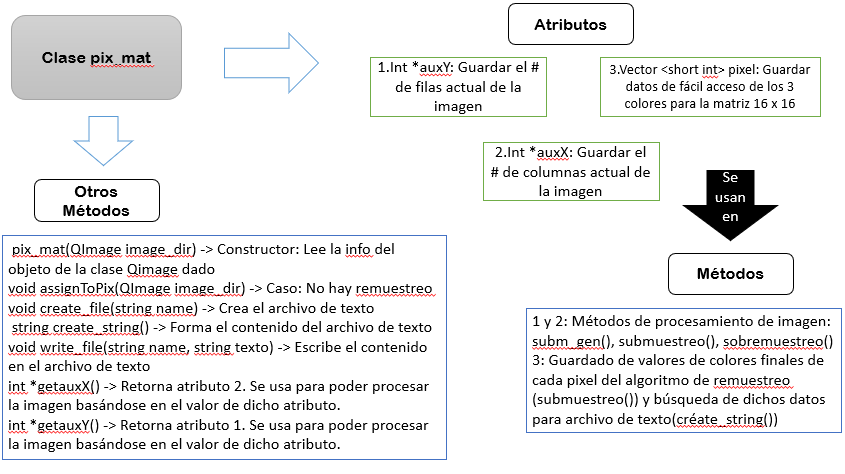
\includegraphics[width=10cm]{pix_mat.png}
    \caption{Clase pix_mat}
    \label{fig:class_pix_mat}
\end{figure}
\begin{figure} 
    \centering
    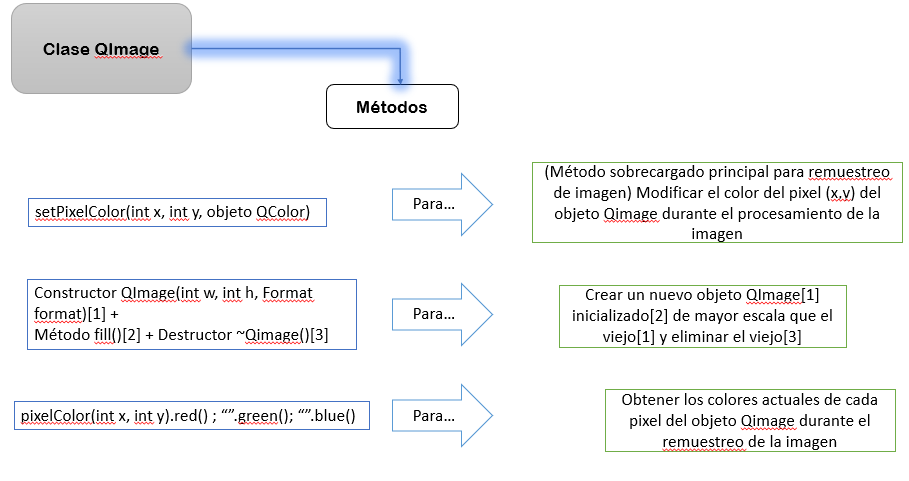
\includegraphics[width=10cm]{QImage.png}
    \caption{Clase QImage}
    \label{fig:class_qimage}
\end{figure}
\begin{figure} 
    \centering
    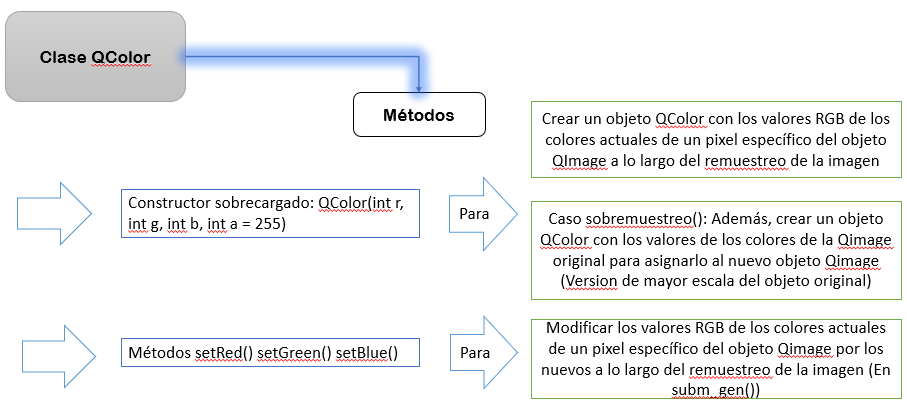
\includegraphics[width=10cm]{QColor.png}
    \caption{Clase QColor}
    \label{fig:class_qcolor}
\end{figure}
\begin{figure} 
    \centering
    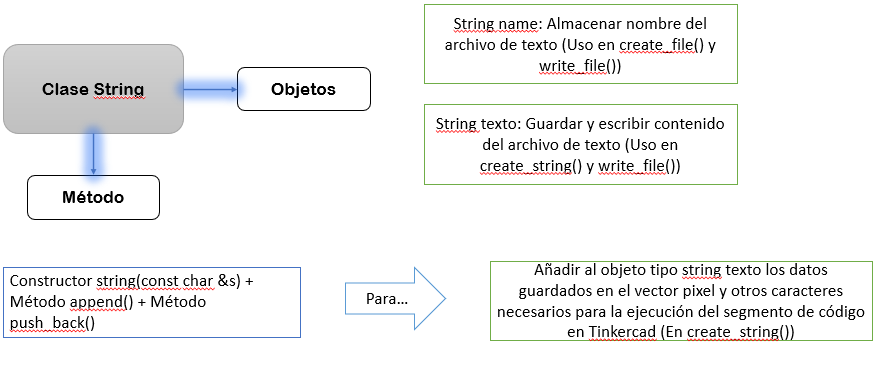
\includegraphics[width=10cm]{String.png}
    \caption{Clase String}
    \label{fig:class_string}
\end{figure}
Otros métodos usados, que no fueron usados, que corresponden más a lo referente con la creación del objeto QImage que almacena la imagen que se encuentra en la dirección que el usuario especifique, corresponde al método de la clase string cstr(), pues con éste se crea un cstring para que sea posible pasarlo como parámetro en la creación del objeto QImage usando el constructor sobrecargado de la clase QImage que recibe la dirección de un archivo. Asimismo, se usaron los métodos width() y height() como referencias para la inicialización de los atributos de la clase pixmat *auxX y *auxY respectivamente (Tanto en el constructor de la clase pixmat como durante el procesamiento de la imagen, en el método de la misma clase submgen()).
El funcionamiento de los métodos y atributos de las clases aquí implementadas se explica en el siguiente apartado dado que su funcionamiento recae principalmente en la interacción entre objetos de las diferentes clases creadas. Los únicos dos módulos de código en el cual la interacción entre las clases sólo se utiliza para el ingreso de los parámetros iniciales y almacenar los valores de salida corresponde al método de la clase pixmat: submuestreo(), cuyos parámetros corresponden a un objeto de la clase QImage, dos punteros *auxX y *auxY, que se asume que tienen los valores actuales del ancho y el alto del objeto de la clase QImage a lo largo del proceso de remuestreo. Pero para ser más precisos, no es como tal que se modifique el ancho y el alto del objeto de la clase QImage en el submuestreo de la imagen, sino que se utiliza la misma matriz de colores RGB en la cual el objeto de la clase QImage guarda los valores de los colores para cada pixel de la imagen. Así, en el caso del método submgen se hace un proceso de submuestreo, llamémoslo de forma general, de modo que en cada iteración del ciclo "while(*auxX >= 64 && *auxY >= 64)" se reduzca a la mitad la cantidad de valores que se deben leer de la matriz de colores RGB del objeto de la clase QImage hasta que su rango se encuentre entre 64 y 127, haciendo a su vez a lo largo de la iteración, un proceso de submuestreo utilizando la lógica de submuestreo por interpolación bilineal cuando se desea reducir una imagen a la mitad de su tamaño actual, principalmente implementado en las siguientes líneas de código de dicho método:
\begin{lstlisting}[language=C++, label=metodopixmat_submgen_interpolacionbilineal]
QColor tipo_color(image_dir.pixelColor(indx/2,indy/2).red(),image_dir.pixelColor(indx/2,indy/2).green(),image_dir.pixelColor(indx/2,indy/2).blue());
if(color == 0){
    tipo_color.setRed((image_dir.pixelColor(indx,indy).red() + image_dir.pixelColor(indx+1,indy).red() + image_dir.pixelColor(indx,indy+1).red() + image_dir.pixelColor(indx+1,indy+1).red())/4);
}
else if(color == 1){
    tipo_color.setGreen((image_dir.pixelColor(indx,indy).green() + image_dir.pixelColor(indx+1,indy).green() + image_dir.pixelColor(indx,indy+1).green() + image_dir.pixelColor(indx+1,indy+1).green())/4);
}
else if(color == 2){
    tipo_color.setBlue((image_dir.pixelColor(indx,indy).blue() + image_dir.pixelColor(indx+1,indy).blue() + image_dir.pixelColor(indx,indy+1).blue() + image_dir.pixelColor(indx+1,indy+1).blue())/4);
}
image_dir.setPixelColor(indx/2,indy/2,tipo_color);
\end{lstlisting}
Y posterior a ello, se reduce el valor de *auxX y *auxY a la mitad, de modo que en la siguiente iteración de dicho código solo se consideren los valores de colores de los pixeles del objeto de la clase QImage que han sido modificados por medio del algoritmo de interpolación bilineal. En cuanto al algoritmo de interpolación bilineal aplicado en el método de la clase pixmat submuestreo(), en la cual, como se aclaró anteriormente, es la única en la que la interacción entre clases sólo se hace al inicio y al final del algoritmo, en éste se entran por parámetro el objeto de la clase QImage, asumiendo que éste ya ha pasado por una primera fase de submuestreo en el método de la clase pixmat submgen(), y los valores actuales de los límites de ancho y alto de la matriz de colores RGB del objeto QImage dentro de los cuales se encuentran los valores enteros de los pixeles de la imagen submuestreada en una primera instancia. Así, en el algoritmo de interpolación bilineal implementado al remuestreo de una imagen de mayor escala a otra de menor con la condición de que la de mayor escala posee un ancho o un alto que no son múltiplos del ancho y el alto de la versión submuestreada de la imagen a la que se desea llegar, se plantea un algoritmo en el cual se plantea como si las dos imágenes estuvieran sobre un mismo plano y la posición de cada pixel correspondiese a una posición en el plano, teniendo en cuenta que los puntos de una misma imagen deben estar a una misma distancia y la suma de las distancias entre punto y punto de la imagen submuestreada debe ser igual a la suma de las distancias entre punto y punto de la imagen original. Asimismo, se debe considerar detalles adicionales como que la imagen submuestreada, por tener una menor cantidad de puntos, implica que en la implementación se considere que se empiecen a ubicar sus respectivos puntos no desde el punto (0,0) hasta el valor de la suma de las distancias entre punto y punto en X y en Y sino desde el punto (mitad de la distancia entre punto y punto en x,mitad de la distancia entre punto y punto en y) hasta el valor de la suma de las distancias entre punto y punto en X y en Y menos la mitad de la distancia entre punto y punto en X y la distancia entre punto y punto en Y respectivamente. Ahora, en el algoritmo en sí, se consideran únicamente los 4 puntos de la imagen actual que son los vecinos más cercanos para un punto A de la imagen submuestreada, de modo que se obtenga la información de la distancia de cada uno de los 4 puntos con respecto al punto A y los valores enteros del color de los 4 pixeles de la imagen actual representados por los 4 puntos(Y así para los 3 colores: Rojo, verde y azul), y posteriormente, emplear el algoritmo de interpolación bilineal, el cual se resume en la siguiente ecuación:
\begin{figure}
    \centering
    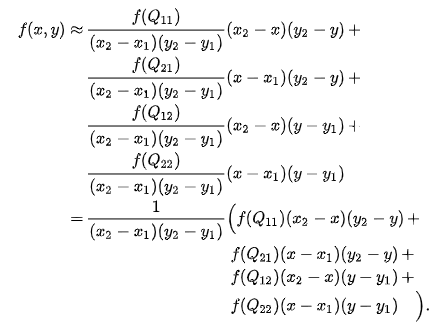
\includegraphics{wikipedia.png}
    \caption{(Extraído de \cite{Wiki_InterpolacionBil})}
    \label{fig:wiki_interpolacionbil}
\end{figure}
Y visto desde el código corresponde principalmente a los siguientes segmentos de código:
\begin{lstlisting}[language=C++, label=code_interpolacionbilineal_part2]
pixel.push_back(short((1/((ix*distOriginX-ix_min*distOriginX)*(iy*distOriginY-iy_min*distOriginY)))*((image_dir.pixelColor(ix_min,iy_min).red()*(ix*distOriginX-(x*dist+dist/2))*(iy*distOriginY-(y*dist+dist/2)))+(image_dir.pixelColor(ix,iy_min).red()*((x*dist+dist/2)-ix_min*distOriginX)*(iy*distOriginY-(y*dist+dist/2)))+(image_dir.pixelColor(ix_min,iy).red()*(ix*distOriginX-(x*dist+dist/2))*((y*dist+dist/2)-iy_min*distOriginY))+(image_dir.pixelColor(ix,iy).red()*((x*dist+dist/2)-ix_min*distOriginX)*((y*dist+dist/2)-iy_min*distOriginY)))));
pixel.push_back(short((1/((ix*distOriginX-ix_min*distOriginX)*(iy*distOriginY-iy_min*distOriginY)))*((image_dir.pixelColor(ix_min,iy_min).green()*(ix*distOriginX-(x*dist+dist/2))*(iy*distOriginY-(y*dist+dist/2)))+(image_dir.pixelColor(ix,iy_min).green()*((x*dist+dist/2)-ix_min*distOriginX)*(iy*distOriginY-(y*dist+dist/2)))+(image_dir.pixelColor(ix_min,iy).green()*(ix*distOriginX-(x*dist+dist/2))*((y*dist+dist/2)-iy_min*distOriginY))+(image_dir.pixelColor(ix,iy).green()*((x*dist+dist/2)-ix_min*distOriginX)*((y*dist+dist/2)-iy_min*distOriginY)))));
pixel.push_back(short((1/((ix*distOriginX-ix_min*distOriginX)*(iy*distOriginY-iy_min*distOriginY)))*((image_dir.pixelColor(ix_min,iy_min).blue()*(ix*distOriginX-(x*dist+dist/2))*(iy*distOriginY-(y*dist+dist/2)))+(image_dir.pixelColor(ix,iy_min).blue()*((x*dist+dist/2)-ix_min*distOriginX)*(iy*distOriginY-(y*dist+dist/2)))+(image_dir.pixelColor(ix_min,iy).blue()*(ix*distOriginX-(x*dist+dist/2))*((y*dist+dist/2)-iy_min*distOriginY))+(image_dir.pixelColor(ix,iy).blue()*((x*dist+dist/2)-ix_min*distOriginX)*((y*dist+dist/2)-iy_min*distOriginY)))));

\end{lstlisting}
Así, como se puede apreciar, el resultado del valor entero del nuevo color obtenido se asigna al vector pixel, el cual es un atributo de la clase pixmat para poder acceder a él después, en el momento en el que se debe armar el contenido del archivo de texto (Lo cual corresponde principalmente a la ejecución del método createstring() de pixmat).
En cuanto a la estructura de la clase implementada en Tinkercad, solo se usa una, la cual corresponde a la de AdafruitNeopixel. Así, se utiliza el constructor de dicha clase para crear un objeto de la misma llamado pixeles pasándole los parámetros de la siguiente forma:
\begin{lstlisting}[language=C++, label=constructor_neopix]
const int pinDatos = 2;
const int numPixeles = 16*16;

Adafruit_NeoPixel pixeles = Adafruit_NeoPixel( numPixeles, pinDatos,
                                              NEO_GRB+NEO_KHZ800);
\end{lstlisting}
Posterior a ello, en la función void setup(), se usa el método de dicha clase begin() para su correcta inicialización. Después, se usa el método setPixelColor() para el objeto pixeles de la clase AdafruitNeopixel, con el objetivo de configurar las 16 tiras de 16 neopixeles del circuito planteado, de tal manera que en los parámetros de dicho método se especifica la posición del neopixel al cual se le desea asignar los 3 valores de los colores RGB indexando el arreglo tipo byte arr de dimensiones 3 x 16 x 16 de la siguiente forma dentro del método setPixelColor():
\begin{lstlisting}[language=C++, label=setpixelcolor_neopix]
pixeles.setPixelColor( 16*i+j, pixeles.Color(arr[0][i][j],arr[1][i][j],arr[2][i][j]));
\end{lstlisting}
En este mismo método, se usa el método Color de la clase AdafruitNeopixel pues el parámetro que debe asignarse en el método setPixelColor() corresponde a su posición y el color formado por la combinación de los valores RGB adjudicados.
\section{Módulos de código implementado donde interactúan las diferentes clases}
El módulo de código implementado donde se da la principal interacción entre clases corresponde al siguiente (main.cpp):
\begin{lstlisting}[language=C++, label=main_interaccion]
    string filename;
    ...
    QImage image_dir(filename.c_str());
    pix_mat matriz_pixeles(image_dir);
    int *auxX = matriz_pixeles.get_auxX();
    int *auxY = matriz_pixeles.get_auxY();
    if(*auxX == 16 && *auxY == 16) matriz_pixeles.assignToPix(image_dir);
    else if(*auxX < 16 || *auxY < 16){
        matriz_pixeles.sobremuestreo(image_dir, auxX, auxY);
    }
    else if(*auxX > 16 && *auxY > 16){
    image_dir = matriz_pixeles.subm_gen(image_dir, auxX, auxY);
    matriz_pixeles.submuestreo(image_dir, auxX, auxY);
    }
    string text = matriz_pixeles.create_string();
    matriz_pixeles.write_file("fileForTinkercad.txt",text);
\end{lstlisting}
Así, primero se crea un objeto filename de la clase string, en el cual se guarda la dirección que el usuario le asigne, se usa el método cstr() de la clase string con dicho objeto, para poder crear un objeto de la clase QImage llamado imagedir con el constructor sobrecargado que recibe la dirección de un archivo. Después se crea el objeto de la clase pixmat matrizpixeles, pasando como parámetro el objeto QImage recién creado, pues sus valores de ancho y alto, obtenidos con los métodos width() y height() respectivamente, son asignados a los atributos del objeto matrizpixeles *auxX y *auxY respectivamente. Además, se crea el archivo de texto en el método de la clase pixmat createfile() usando un objeto de la clase string pero sin interactuar con otras clases dentro de dicho método.
\begin{lstlisting}[language=C++, label=asignar_atributospixmat]
    create_file("fileForTinkercad.txt");
    auxX = new int;
    auxY = new int;
    *auxX = image_dir.width();
    *auxY = image_dir.height();
\end{lstlisting}
Una vez asignados, se obtienen dichos atributos del objeto matrizpixeles con los métodos getauxX() y getauxY de la clase pixmat para asignárselos a los punteros de tipo entero *auxX y *auxY, en caso de que sean iguales a 16, no es necesario hacer un proceso de remuestreo de la imagen, por lo cual se usa el método de la clase pixmat assignToPix(), entrando por parámetro el objeto imagedir tipo QImage, para agregar, con el método pushback() del contenedor vector, al atributo vector <short int> pixel del objeto matrizpixeles los valores enteros de cada color (Rojo, verde y azul) de cada pixel de la imagen, que se obtienen usando los métodos pixelColor(int x, int y).red(), pixelColor(int x, int y).green() y pixelColor(int x, int y).blue() teniendo en cuenta los valores de los atributos *auxX y *auxY.
\begin{lstlisting}[language=C++, label = assigntopix]
    for(int y = 0; y < *auxY; y++){
        for(int x = 0; x < *auxX; x++){
            pixel.push_back(short(image_dir.pixelColor(x,y).red()));
            pixel.push_back(short(image_dir.pixelColor(x,y).green()));
            pixel.push_back(short(image_dir.pixelColor(x,y).blue()));
        }
    }
\end{lstlisting}
En caso de que se identifique que el *auxX o *auxY son menores que 16, se ejecuta el método sobremuestreo() para el objeto matrizpixeles tipo pixmat pasando por parámetro el objeto imagedir tipo QImage y los punteros auxX y auxY creados. Dentro de este método, se crea con el constructor sobrecargado de la clase QImage un objeto llamado image con dimensiones 16 veces mayores que las de la original y se usa el método fill() de la clase QImage para incializar el objeto con unos valores predeterminados, de modo que como parámetro de dicho método se pasa un objeto tipo QColor con valores RGB de (1,1,1). Posterior a ello, se asigna a cada uno de los pixeles del nuevo objeto image tipo QImage, por medio del método de dicha clase setPixelColor(), los mismos colores que los del objeto imagedir tipo QImage, teniendo en cuenta que debe ser el mismo color para cada matriz de 16 x 16 dentro del nuevo objeto QImage creado con el objetivo de que este nuevo objeto sea una versión de mayor escala del objeto imagedir tipo QImage. Por tal razón, se usa a su vez, en el objeto imagedir, los métodos pixelColor(x,y).red(), pixelColor(x,y).blue() y pixelColor(x,y).green() para obtener sus colores en una posición determinada. Y así, crear un objeto QColor con su constructor sobrecargado QColor(int r, int g, int b, int a = 255) con los valores obtenidos, pues éste se debe pasar como parámetro para el método sobrecargado setPixelColor(x,y,objeto tipo QColor). Dado que la imagen original no se va a volver a tener en cuenta en el resto del proceso de remuestreo, se elimina el objeto imagedir tipo QImage con su respectivo destructor.
(Se hace la aclaración de que el proceso de aquí en adelante es similar para el caso en el que *auxX y *auxY son mayores que 16, con la diferencia de que el objeto imagedir tipo QImage no es eliminado y es usado para el proceso de remuestreo en lugar de usar el objeto image tipo QImage como se hace para el caso que toque hacer sobremuestreo)
Después se emplea el método submgen de la clase pixmat pasando como parámetro el nuevo objeto tipo QImage image y los punteros *auxX y *auxY. Dentro de submgen, la principal interacción se da entre las clases QColor y QImage, de modo que se crea en cada ciclo un objeto tipo QColor llamado tipocolor con los valores actuales de rojo, verde y azul de un pixel de la imagen, usando como referencia lo que retorna para el objeto imagedir los métodos pixelColor().red(), pixelColor().green() y pixelColor().blue() de la clase QImage y, después, empleando la lógica de interpolación bilineal explicada en el anterior apartado, se utilizan en el objeto tipocolor los métodos setRed(), setGreen() y setBlue() para modificar los colores del objeto tipocolor y,posteriormente, pasar dicho objeto como parámetro del método setPixelColor sobrecargado: setPixelColor(int x, int y, objeto tipo QColor) usándolo con el objeto imagedir.
Una vez hecho este proceso, se retorna el objeto imagedir tipo QImage y se asigna con el operador sobrecargado = al objeto image que ya estaba creado en el método sobremuestreo() de la clase pixmat. Después, este objeto image se pasa como parámetro del método submuestreo() de la clase pixmat, donde se hace el proceso de submuestreo del objeto image tipo QImage creado, explicado en el anterior apartado, y se asignan los resultados de dicho proceso al atributo del objeto matrizpixeles de la clase pixmat.
Ahora, se ejecuta el segmento de código: 
\begin{lstlisting}[language=C++, label=method_createstring]
string text = matriz_pixeles.create_string();
\end{lstlisting}
En el cual se crea un objeto text de la clase string que recibe el objeto tipo string que retorna el método createstring() de la clase pixmat, empleado para el objeto matrizpixeles. Dentro de este método, se recorre el contenedor vector pixel del objeto matrizpixeles 3 veces, dado que se deben únicamente extraer los valores enteros de un color específico en cada iteración, y son agregados al contenido del objeto texto tipo string, junto con otros caracteres, que contiene la línea de código que se debe añadir en el proyecto de Tinkercad. Todos los valores enteros extraídos del atributo pixel del objeto matrizpixeles son agregados al objeto texto tipo string por medio del método pushback() de la clase string, mientras que los otros caracteres son agregados tanto por este medio como mediante el método de la clase string append(), pasando como parámetro un objeto tipo string creado con el constructor sobrecargado que permite pasar como parámetro una serie de caracteres constantes (const char) previamente definidos.
Una vez se ha asignado el objeto texto tipo string al objeto text tipo string, se procede a ejecutar la siguiente línea de código:
\begin{lstlisting}[language=C++, label=method_writefile]
matriz_pixeles.write_file("fileForTinkercad.txt",text);
\end{lstlisting}
En la cual se usa el método writefile() de la clase pixmat para el objeto matrizpixeles, en la cual se pasan como parámetros dos strings: El primero de ellos contiene una serie de caracteres constantes que corresponden al nombre con su extensión del archivo de texto mientras el segundo almacena el contenido que se debe agregar al archivo de texto. Dentro de dicho método no hay una interacción entre las clases utilizadas, sólo se usan los strings pasados por parámetro.
En cuanto al código en Tinkercad, sólo se hace uso de una única clase de la librería AdafruitNeopixel.h. Por lo cual no hay interacción con otras clases.
\section{Estructura del circuito montado}
En caso de modificaciones, el último montaje de la matriz de Neopixeles es la versión final del proyecto en Tinkercad. La primera versión corresponde a una matriz de Neopixeles de 8 x 8 en la cual se usa el pin digital 2 del Arduino Uno como pin de salida para transmitir la información leída del archivo de texto y guardada en un arreglo tridimensional de valores enteros, usando los métodos de la librería correspondiente de dichos componentes para su efectiva configuración a partir del uso del pin 2 del Arduino Uno. En esta matriz, a pesar de estas dispuestos como tiras de 8 neopixeles una después de la otra en el eje y, en cuanto a conexiones, están conectados de modo que la entrada de la tira de la fila superior está conectada en su puerto de entrada al pin 2 y su puerto negativo y positivo conectado al negativo y positivo, respectivamente, de un suministro de energía, el cual está configurado para transmitir un voltaje máximo de 5 voltios y una corriente máxima de 20 amperios dado que el máximo que pueden soportar las tiras de neopixeles es de 5.5 voltios basándose en los recuadros de advertencia que muestra Tinkercad al subir el voltaje que suministra dicho componente. Dicho suministro de energía se encuentra conectado, en su puerto negativo, con el puerto negativo del Arduino Uno. Los segundos puertos de positivo, negativo y el puerto de salida están conectados, respectivamente, a los puertos positivo, negativo y de entrada de la tira de 8 neopixeles de la fila inferior a ella. Y así sucesivamente hasta llegar a la tira de neopixeles de la última fila, cuyo puerto de salida, uno de los positivos y uno de los negativos se encuentra desconectado pues corresponde a la última fila. En primera instancia, se espera que, en dado caso que se modifique el circuito, no implique un cambio en las conexiones del circuito drásticamente, sino únicamente en la cantidad de neopixeles que se desea usar por fila y/o columna.
\begin{figure} 
    \centering
    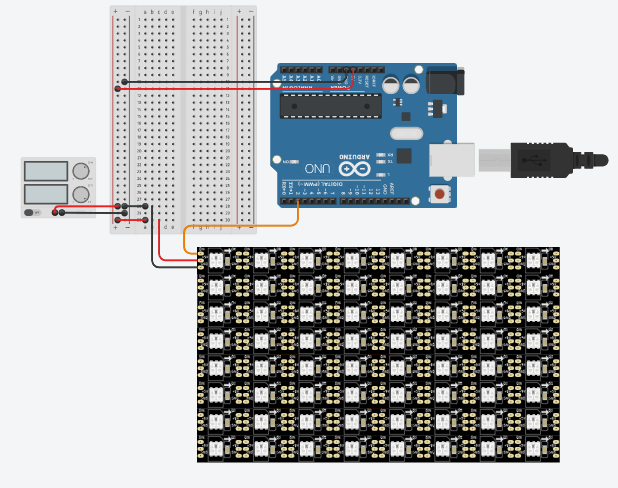
\includegraphics[width=10cm]{matriz8x8Neopixeles.png}
    \caption{Matriz de 8 x 8 Neopixeles}
    \label{fig:mat8x8_neo}
\end{figure}
En efecto, se hizo un cambio en la estructura del circuito montado, pero, como se había esperado anteriormente, únicamente implicó un cambio en la cantidad de neopixeles asignados para cada fila y para cada columna (16 x 16), pero en cuanto a la lógica de conexión entre tiras de neopixeles y entre la primera tira y el suministro de energía, a su vez que el suministro de neergía se encuentra conectado a la tarjeta de Arduino Uno es la misma planteada inicialmente.
\begin{figure} 
    \centering
    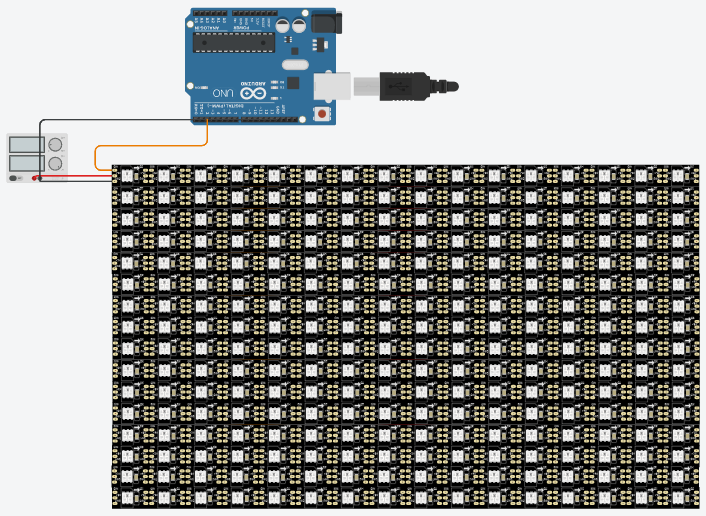
\includegraphics[width=10cm]{matriz16x16.png}
    \caption{Matriz de 16 x 16 Neopixeles}
    \label{fig:mat16x16_neo}
\end{figure}
\section{Problemas presentados durante la implementación}
Al realizar pruebas con código en el proyecto en Tinkercad, en primer lugar, hubo una serie de problemas al usar un buffer de un tamaño lo suficientemente grande para que el usuario ingresase línea por línea el contenido del archivo de texto de tal modo que cada línea representara una de las filas de la matriz, con el fin de que el usuario tenga que hacer el menor esfuerzo posible, no fue viable debido a que al usar tanto memoria en Stack como por memoria dinámica, el buffer solo alcanzaba a captar un poco más de la mitad de la línea que se ingresaba por medio del monitor en serie, por lo cual decidí que tocaba hacer que cada línea representara la información de los 3 colores de 4 neopixeles de una misma fila, de modo que por cada 2 ingresos de datos, se cambia el número de la fila. Dicha información ingresada por el usuario es almacenada en una matriz tridimensional de enteros llamada "pixeles", la cual va a ser indexada con el objetivo de configurar los neopixeles con el método "setPixelColor" que proporciona la librería de Adafruit Neopixel. De esta forma, se configuró todo dentro de una función, además de organizar dentro de una función las instrucciones que se le dan al usuario una vez termina de representar su bandera así como cuando inicializa el programa. De la misma forma, se creó una función para que el usuario tenga la opción de verificar el correcto funcionamiento de los neopixeles de la matriz de 8 x 8. A continuación, la primera versión organizada del código en Tinkercad descrito anteriormente:
\begin{lstlisting}[language=C++, label=prueba_ingresotxtymanualgeneraltink]
#include <Adafruit_NeoPixel.h>

#define LED_PIN 2

#define LED_COUNT 64

Adafruit_NeoPixel leds(LED_COUNT, LED_PIN, NEO_GRB + NEO_KHZ800);

void verificacion();
void ingreso_info();
void main_instruc();

void setup()
{
  leds.begin();
  Serial.begin(9600);
  int pixeles[3][LED_COUNT/8][LED_COUNT/8] = {0};
  main_instruc();
}

void loop()
{
  if(Serial.available()>0){
    int numero = Serial.parseInt();
    if(numero == 1){
      verificacion();
    }
    else if(numero == 2){
      Serial.println("Por favor, ingrese en el monitor en serie el contenido del archivo");
      Serial.println("de texto dado en el primer programa usado ingresando linea por linea,");
      Serial.println("(Es decir el archivo de texto que se le menciono mantener abierto para este segundo programa");
      Serial.println("exactamente como se encuentra escrito. No modifique nada del contenido.");
      Serial.println("En el monitor en serie, se le va a mostrar un aviso para poder copiar 1 linea");
      Serial.println("y pegarla en el recuadro del monitor en serie, en su parte inferior, habilitado para pegar dicha linea.");
      Serial.println("Una vez verifique que la linea ha sido copiada y pegada correctamente, oprima enter para ingresarla.");
      Serial.write("\n\n\n");
      ingreso_info();
      main_instruc();
    }
    else{
      Serial.println("El numero ingresado no se encuentra entre las opciones dadas.");
      Serial.println("Por favor, ingrese otro numero.");
      main_instruc();
    }
  }
}

void main_instruc(){
  Serial.println("Estimado cliente, para hacer uso de esta matriz de neopixeles,");
  Serial.println("por favor, en el monitor en serie, escriba:");
  Serial.println("1 para verificar el correcto funcionamiento de la matriz");
  Serial.println("2 para representar en la matriz la imagen de la bandera escogida en el anterior programa");
}

void verificacion(){
  Serial.println("Verificacion de Matriz de Neopixeles 8 x 8");
  for(int i = 0; i < LED_COUNT; i += 1){
    leds.setPixelColor(i, 207, 97, 62);
  }
  leds.show();
  delay(3000);
  Serial.println("Finalizando Verificacion...");
  for(int i = 0; i < LED_COUNT; i += 1){
    leds.setPixelColor(i, 0, 0, 0);
  }
  leds.show();
}

void ingreso_info(){
  int *ptr_cont= NULL;
  ptr_cont = new int;
  *ptr_cont = 0;
  int num_color = 0, f = 0, c = 0;
  while(*ptr_cont <= 15){
    delay(1000);
    if(Serial.available()>0){
      const int length = 48;
      char *fil = new char[length];
      int user = Serial.readBytes(fil,length);
      int valColor[3] = {0};
      for(int i = 0; i<=length-1; i++){
        Serial.println(int(fil[i]));
        if(int(fil[i]) == 44){ // ,
          num_color++;
          int col = 0;
          for(int i = 2; i>=0; i--){
            int mult = 1;
            if(valColor[i] != 46){ // No hay mas .
              col = col + (valColor[i]-48)*mult;
              mult = mult*10;
            }
            pixeles[num_color][f][c] = col; //Asignacion color
          }
          
        }
        else if(int(fil[i]) == 59){ // ;
          for(int i = 0; i<=2;i++) valColor[i] = 0;
          num_color = 0;
          c++;
        }
      }
      delete[] fil;
      if(*ptr_cont%2!=0){
        f++;
        c=0;
      }
      *ptr_cont = *ptr_cont + 1;
    }
  }
  delete [] ptr_cont;
}
\end{lstlisting}
Dicho código tenía unos fallos en cuanto al uso de memoria e indexaciones hechas de manera errónea, por lo cual se hizo una serie de modificaciones para mejorar este aspecto, no obstante aún se mantiene un problema de guardado de cantidades enteras erróneas y, en adición a esto, parte del código se está ejecutando más veces de las que se tiene previsto, haciendo que la cantidad de colores que se va a guardar para cada pixel sea de 5 en vez de 3.
\begin{lstlisting}[language=C++, label=error_guardarints]
#include <Adafruit_NeoPixel.h>

#define LED_PIN 2

#define LED_COUNT 64

Adafruit_NeoPixel leds(LED_COUNT, LED_PIN, NEO_GRB + NEO_KHZ800);

void verificacion();
void ingreso_info();
void main_instruc();

int pixeles[3][LED_COUNT/8][LED_COUNT/8] = {0};

void setup()
{
  leds.begin();
  Serial.begin(9600);
  main_instruc();
}

void loop()
{
  if(Serial.available()>0){
    int numero = Serial.parseInt();
    if(numero == 1){
      verificacion();
    }
    else if(numero == 2){
      Serial.println("Por favor, ingrese en el monitor en serie el contenido del archivo");
      Serial.println("de texto dado en el primer programa usado ingresando linea por linea,");
      Serial.println("(Es decir el archivo de texto que se le menciono mantener abierto para este segundo programa");
      Serial.println("exactamente como se encuentra escrito. No modifique nada del contenido.");
      Serial.println("En el monitor en serie, se le va a mostrar un aviso para poder copiar 1 linea");
      Serial.println("y pegarla en el recuadro del monitor en serie, en su parte inferior, habilitado para pegar dicha linea.");
      Serial.println("Una vez verifique que la linea ha sido copiada y pegada correctamente, oprima enter para ingresarla.");
      Serial.write("\n\n\nIngrese la primera linea.");
      ingreso_info();
      main_instruc();
    }
    else{
      Serial.println("El numero ingresado no se encuentra entre las opciones dadas.");
      Serial.println("Por favor, ingrese otro numero.");
      main_instruc();
    }
  }
}

void main_instruc(){
  Serial.println("Estimado cliente, para hacer uso de esta matriz de neopixeles,");
  Serial.println("por favor, en el monitor en serie, escriba:");
  Serial.println("1 para verificar el correcto funcionamiento de la matriz");
  Serial.println("2 para representar en la matriz la imagen de la bandera escogida en el anterior programa");
}

void verificacion(){
  Serial.println("Verificacion de Matriz de Neopixeles 8 x 8");
  for(int i = 0; i < LED_COUNT; i += 1){
    leds.setPixelColor(i, 207, 97, 62);
  }
  leds.show();
  delay(3000);
  Serial.println("Finalizando Verificacion...");
  for(int i = 0; i < LED_COUNT; i += 1){
    leds.setPixelColor(i, 0, 0, 0);
  }
  leds.show();
}

void ingreso_info(){
  int *ptr_cont= NULL, *num_color = NULL, *f = NULL, *c = NULL;
  ptr_cont = new int, num_color = new int, f = new int, c = new int;
  *ptr_cont = 0, *num_color = 0, *f = 0, *c = 0;
  while(*ptr_cont <= 15){
  	delay(500);
    if(Serial.available()>0){
    	const int length = 48;
    	char *fil = new char[length];
      	int user = Serial.readBytes(fil,length);
      	int valColor[3] = {0};
      	for(int i = 0; i<=length-1; i++){
        	if(int(fil[i]) == 44){ // ,
          		int col = 0, mult = 1;
          		for(int i = 2; i >=0; i--){
            		if(valColor[i] != 46){ // No hay mas .
              			col = col + (valColor[i]-48)*mult;
              			mult = mult*10;
            		}
                }
              	Serial.print(*num_color);
                Serial.print(",");
                Serial.print(*f);
                Serial.print(",");
                Serial.print(*c);
                Serial.print("=");
                Serial.println(col);
              	pixeles[*num_color][*f][*c] = col; //Asignacion color
                for(int i = 0; i<=2;i++){
                	valColor[i] = 0;
              	}
              	*num_color= 1+*num_color;
    	    }
        	else if(int(fil[i]) == 59){ // ;
              	int col = 0, mult = 1;
          		for(int i = 2; i >=0; i--){
            		if(valColor[i] != 46){ // No hay mas .
              			col = col + (valColor[i]-48)*mult;
              			mult = mult*10;
            		}
                Serial.print(*num_color);
                Serial.print(",");
                Serial.print(*f);
                Serial.print(",");
                Serial.print(*c);
                Serial.print("=");
                Serial.println(col);
            	pixeles[*num_color][*f][*c] = col; //Asignacion color
                *num_color = 10+*num_color;
                }
              	for(int i = 0; i<=2;i++){
                	valColor[i] = 0;
              	}
          		*num_color = 0;
          		*c = 1 + *c;
        	}
            else{
            	valColor[i%4] = int(fil[i]);
            }
      	}
      	for(int i = 0; i<=length-1; i++){
        	//Serial.println(int(fil[i]));
        }
      	if(*ptr_cont!=15){
        	Serial.println("Ingrese la siguiente linea.");
      	}
      	if(*ptr_cont%2!=0){
          		*f = 1 + *f;
          		*c=0;
       	}
      	delete[] fil;
	    *ptr_cont = *ptr_cont + 1;
    }
  }
  delete [] ptr_cont, num_color, f, c;
}
\end{lstlisting}
Una vez resuelto dicho problema, se procedió a la creación de la función representar(), la cual se encarga de la representación de los valores enteros extraídos del archivo de texto, ahora guardados en el arreglo tridimensional de enteros "pixeles". No obstante, surgió un nuevo problema con la función verificación, pues, a pesar de no tener modificaciones en ningún aspecto, se comenzó a presentar fallas en la representación del color asignado para mostrar en todos los neopixeles de la matriz, esto hecho con el objetivo de que esto mostrase que, efectivamente, es funcional. De la misma forma, este problema se presentó cuando se trató de configurar los neopixeles de la matriz dentro de la función representar(). A pesar de ello, se pudo confirmar que tanto el guardado de la información como la indexación de los valores del arreglo "pixeles" fueron exitosos, por lo cual este sería el último problema aparente por resolver en cuanto a la parte de Tinkercad:
\begin{lstlisting}[language=C++, label=error_electronica]
#include <Adafruit_NeoPixel.h>

#define LED_PIN 2

#define LED_COUNT 64

Adafruit_NeoPixel leds(LED_COUNT, LED_PIN, NEO_GRB + NEO_KHZ800);

void verificacion();
void ingreso_info();
void representar();
void main_instruc();

int pixeles[3][LED_COUNT/8][LED_COUNT/8] = {0};

void setup()
{
  leds.begin();
  Serial.begin(9600);
  main_instruc();
}

void loop()
{
  if(Serial.available()>0){
    int numero = Serial.parseInt();
    if(numero == 1){
      verificacion();
    }
    else if(numero == 2){
      Serial.println("Por favor, ingrese en el monitor en serie el contenido del archivo");
      Serial.println("de texto dado en el primer programa usado ingresando linea por linea,");
      Serial.println("(Es decir el archivo de texto que se le menciono mantener abierto para este segundo programa");
      Serial.println("exactamente como se encuentra escrito. No modifique nada del contenido.");
      Serial.println("En el monitor en serie, se le va a mostrar un aviso para poder copiar 1 linea");
      Serial.println("y pegarla en el recuadro del monitor en serie, en su parte inferior, habilitado para pegar dicha linea.");
      Serial.println("Una vez verifique que la linea ha sido copiada y pegada correctamente, oprima enter para ingresarla.");
      Serial.write("\n\n\nIngrese la primera linea.");
      ingreso_info();
      representar();
      main_instruc();
    }
    else{
      Serial.println("El numero ingresado no se encuentra entre las opciones dadas.");
      Serial.println("Por favor, ingrese otro numero.");
      main_instruc();
    }
  }
}

void main_instruc(){
  Serial.println("Estimado cliente, para hacer uso de esta matriz de neopixeles,");
  Serial.println("por favor, en el monitor en serie, escriba:");
  Serial.println("1 para verificar el correcto funcionamiento de la matriz");
  Serial.println("2 para representar en la matriz la imagen de la bandera escogida en el anterior programa");
}

void verificacion(){
  Serial.println("Verificacion de Matriz de Neopixeles 8 x 8");
  for(int i = 0; i < LED_COUNT; i += 1){
    leds.setPixelColor(i, 207, 97, 62);
  }
  leds.show();
  delay(3000);
  Serial.println("Finalizando Verificacion...");
  for(int i = 0; i < LED_COUNT; i += 1){
    leds.setPixelColor(i, 0, 0, 0);
  }
  leds.show();
}

void ingreso_info(){
  int *ptr_cont= NULL, *num_color = NULL, *f = NULL, *c = NULL;
  ptr_cont = new int, num_color = new int, f = new int, c = new int;
  *ptr_cont = 0, *num_color = 0, *f = 0, *c = 0;
  while(*ptr_cont <= 15){
  	delay(500);
    if(Serial.available()>0){
    	const int length = 48;
    	char *fil = new char[length];
      	int user = Serial.readBytes(fil,length);
      	int valColor[3] = {0};
      	for(int i = 0; i<=length-1; i++){
        	if(int(fil[i]) == 44){ // ,
          		int col = 0, mult = 1;
          		for(int i = 2; i >=0; i--){
            		if(valColor[i] != 46){ // No hay mas .
              			col = col + (valColor[i]-48)*mult;
              			mult = mult*10;
            		}
                }
              	/*Serial.print(*num_color);
                Serial.print(",");
                Serial.print(*f);
                Serial.print(",");
                Serial.print(*c);
                Serial.print("=");
                Serial.println(col);*/
              	pixeles[*num_color][*f][*c] = col; //Asignacion color
              	*num_color= 1+*num_color;
    	    }
        	else if(int(fil[i]) == 59){ // ;
              	int col = 0, mult = 1;
          		for(int i = 2; i >=0; i--){
            		if(valColor[i] != 46){ // No hay mas .
              			col = col + (valColor[i]-48)*mult;
              			mult = mult*10;
            		}
                }
                /*Serial.print(*num_color);
                Serial.print(",");
                Serial.print(*f);
                Serial.print(",");
                Serial.print(*c);
                Serial.print("=");
                Serial.println(col);*/
            	pixeles[*num_color][*f][*c] = col; //Asignacion color
          		*num_color = 0;
          		*c = 1 + *c;
        	}
            else{
            	valColor[i%4] = int(fil[i]);
            }
      	}
      	if(*ptr_cont!=15){
        	Serial.println("Ingrese la siguiente linea.");
      	}
      	if(*ptr_cont%2!=0){
          		*f = 1 + *f;
          		*c=0;
       	}
      	delete[] fil;
	    *ptr_cont = *ptr_cont + 1;
    }
  }
  delete [] ptr_cont, num_color, f, c;
}
void representar(){
  	int *neo_indx = new int;
    for(int fil = 0; fil < LED_COUNT/8; fil++){
       	for(int col = 0; col < LED_COUNT/8; col++){
            leds.setPixelColor(*neo_indx,pixeles[0][fil][col],pixeles[1][fil][col],pixeles[2][fil][col]);
          	int red = pixeles[0][fil][col];
          	int green = pixeles[1][fil][col];
          	int blue = pixeles[2][fil][col];
          	Serial.println(red);
        	Serial.println(green);
         	Serial.println(blue);
          	Serial.println();
        	*neo_indx = *neo_indx + 1;
        }
      	*neo_indx = *neo_indx + 1;
    }
  	leds.show();
  	delete [] neo_indx;
}
\end{lstlisting}
Después de una serie de pruebas, se plantea que uno de los problemas constituye el hecho de no poder hacer que el usuario ingrese una menor cantidad de líneas, para que haga el menor esfuerzo. Por tal razón, se procede a buscar métodos para facilitar el ingreso de datos. Otro problema, esta vez en Qt, correspondió a la lectura errónea de los pixeles de una imagen pequeña dada en formato jpg, por lo cual se estableció que, para imagenes con un alto o ancho menor a 100 pixeles sea necesario que su formato sea en PNG, pues, después de hacer pruebas con imágenes dadas en dicho formato, fueron leídas sin presentar estos mismos problemas, asimismo, al hacer pruebas usando el debugger y usar comandos para ver en la terminal los datos de la imagen, los datos dados en la terminal variaban con respecto a los que se obtenían a cuando se corría el programa de manera normal. Así, para imágenes que no cumplan dichas condiciones (Mayores o iguales a 100 pixeles en ancho y alto), su formato debe ser en JPG, pues no hay problema alguno en este caso.
En cuanto a problemas en el código en Qt referentes al algoritmo de submuestreo y sobremuestreo, en la función submgen no hubo mayor problema pues se siguió la lógica planteada en las referencias del informe de diseño de la presente solución al problema.
En la función submuestreo, se siguió una lógica similar, pero esta vez un poco más compleja debido a que las magnitudes del ancho y el alto de la imagen resultante en la función submgen, como caso general, no eran múltiplos de 8 (Pues 8 corresponde al valor tanto del ancho como del alto de la matriz de neopixeles).
En cuanto a la función sobremuestreo, dado que se planteó que sólo había que reescalar la imagen de forma manual y después hacer a dicha imagen un proceso de submuestreo, el principal problema radicó en el hecho de no poder identificar a simple vista que el problema no era a causa del código planteado sino del formato especificado en las instrucciones dadas. A pesar de que el desafío planteado especifica que es obligatorio recibir un formato jpg, se concluyó que éste método, para el caso de imágenes que sean de un tamaño pequeño, resulta inefectivo al momento de hacer la lectura de sus pixeles uno a uno, en el caso de que el usuario cree una imagen en formato jpg usando programas como paint, que reeditan los colores de la imagen originalmente dados. Por esta razón, además de la otra mencionada anteriormente, después de un límite mínimo de ancho y alto, se le recomienda al usuario que la imagen ingresada sea en formato png.
Uno de los problemas que sí tomó tiempo más que dificultad consistió en el hecho de que no había comprendido el hecho de que no tocaba ingresar el código por el monitor serial sino que era copiar y pegar el contenido directamente en el código de Tinkercad, por lo cual las pruebas anteriores que hice tratando de usar buffers para que el usuario ingresase la información fueron desechos en su totalidad y el código final en Tinkercad pasó a ser más simple. Asimismo tocó modificar en el método de la clase pixmat que se encargaban de modificar el objeto de la clase string usado para almacenar el contenido del archivo de texto que hay que llevar a la parte de Tinkercad. Así, en Tinkercad, de pasar de esa versión final se pasó a la siguiente versión: 
\begin{lstlisting}[language=C++, label=final_tinker]
#include <Adafruit_NeoPixel.h>

const int pinDatos = 2;
const int numPixeles = 16*16;

Adafruit_NeoPixel pixeles = Adafruit_NeoPixel( numPixeles, pinDatos,
                                              NEO_GRB+NEO_KHZ800);
void setup()
{
  pixeles.begin();

  for(unsigned int i = 0; i < 16; i++){
    for(unsigned int j = 0; j < 16; j++){
      pixeles.setPixelColor( 16*i+j, pixeles.Color(arr[0][i][j],arr[1][i][j],arr[2][i][j]));
    }
  }
  pixeles.show();
}
void loop()
{
  
}
\end{lstlisting}
Así, en la segunda línea del código mostrado anteriormente, es el lugar donde se le indica al usuario que debe pegar el contenido del archivo de texto resultante del procesamiento de la imagen con el programa hecho en Qt.
En cuanto al cambio de una matriz de 8 x 8 a una de 16 x 16, fue sólo cuestión de cambiar unos pequeños datos para que no se trabajaran los datos para redimensionar la imagen a una de 8 x 8 sino a una de 16 x 16 pixeles, pero no algo complejo como verificar el algoritmo entero, por lo cual no representó mayor problema. Pues en los algoritmos, el valor del número de columnas y el de filas de la matriz sólo son empleados como puntos de referencia para iniciar la lógica del algoritmo así como los límites que debe tener el número de vectores a crear una vez el algoritmo tiene el valor que debe asignar para un pixel en específico. La razón por la cual se hizo dicho cambio fue debido a que, al representar en una matriz de 8 x 8, la forma en cómo se veía la bandera en la matriz de neopixeles difería en ciertos casos en filas o columnas enteras. No obstante, he de decir que esto también puede presentarse en una matriz de 16 x 16, sin embargo, es menos probable dado que la cantidad de neopixeles disponibles para representar la matriz es mayor. Asimismo, no se toman valores más grandes a 16 como el valor de las columnas o las filas de neopixeles dado que, mediante pruebas hechas con imágenes para su sobremuestreo, dada la lógica de sobremuestreo planteada, resulta inefectivo tomar valores mayores a este número. De la misma forma, en todo momento se plantea que el número de filas debe ser igual al número de columnas dado que la libertad para una matriz cuadrada es mayor en comparación con una matriz rectangular, es decir, si se tiene por ejemplo una matriz rectangular de 16 x 12, dado el mejor caso en el que las filas sean múltiplo de 16 y las columnas sea múltiplo de 12, dado el algoritmo planteado, la representación se realiza con mayor facilidad, no obstante para casos diferentes a este, la representación resulta más compleja en comparación con una matriz cuadrada debido a que, dado el algoritmo creado, es de mayor probabilidad que se ignoren valores de la imagen original que, en una matriz cuadrada, tienen mayor probabilidad de considerar dentro de un algoritmo basado en la interpolación bilineal, teniendo en cuenta que dicho algoritmo se fundamenta en el análisis de 4 puntos de la matriz que forman un cuadrado. En otras palabras, no es que una matriz cuadrada sea drásticamente mejor que una matriz rectangular, pero basándome en las pruebas realizadas, considero que una matriz cuadrada se puede enfocar en mejorar los casos promedio de la representación de una bandera en compensación de sacrificar parte de la calidad para el mejor caso, que considero es el enfoque de una matriz rectangular.

\bibliographystyle{IEEEtran}
\bibliography{references}
\end{document}